\chapter{}

\section{引言}

\section{旋转机械故障诊断}

\begin{figure}[!htbp]
    \centering
    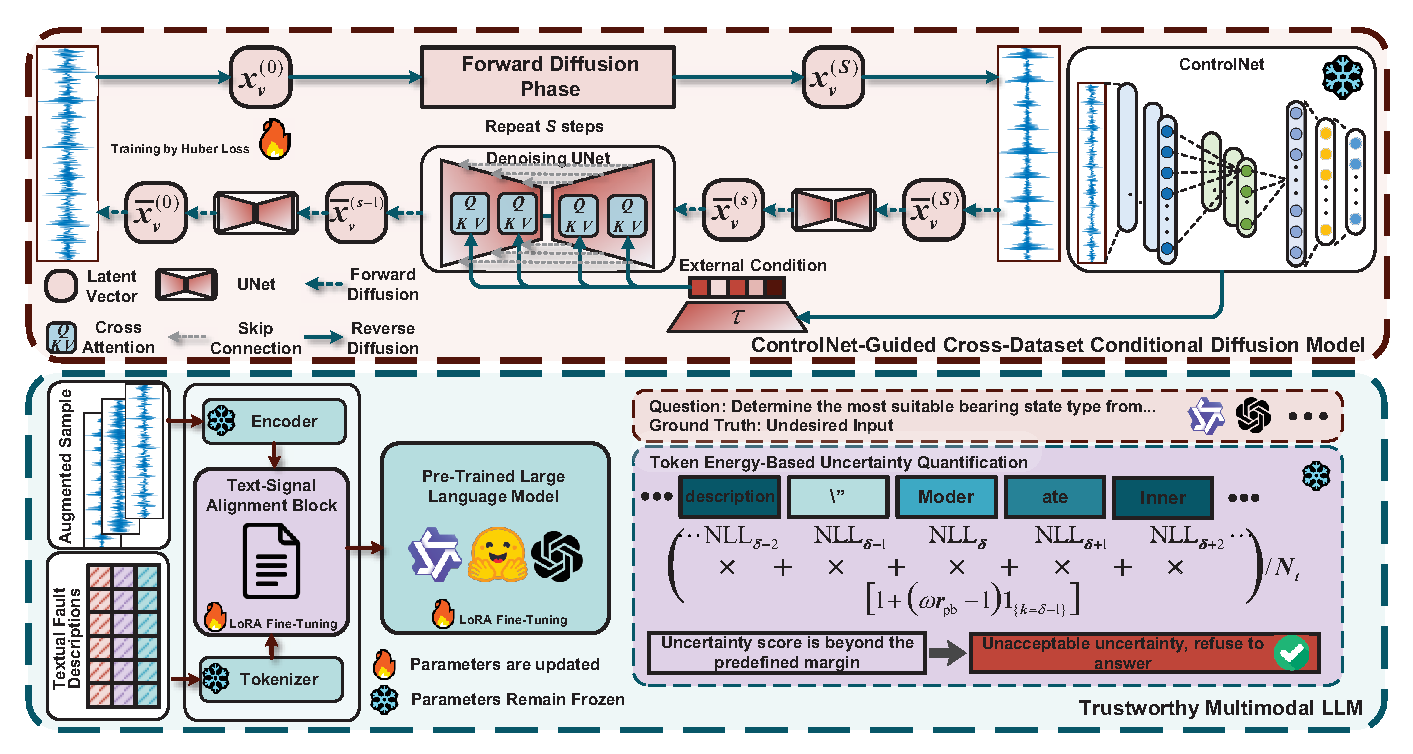
\includegraphics[width=\textwidth]{Img/DA-TMLLM_figures/trans/whole_framework.eps}
    \bicaption{DA-TMLLM~架构图}{Diagram of DA-TMLLM framework}
    \label{fig:da-tmllm_framework}
\end{figure}

\begin{figure}[!htbp]
    \centering
    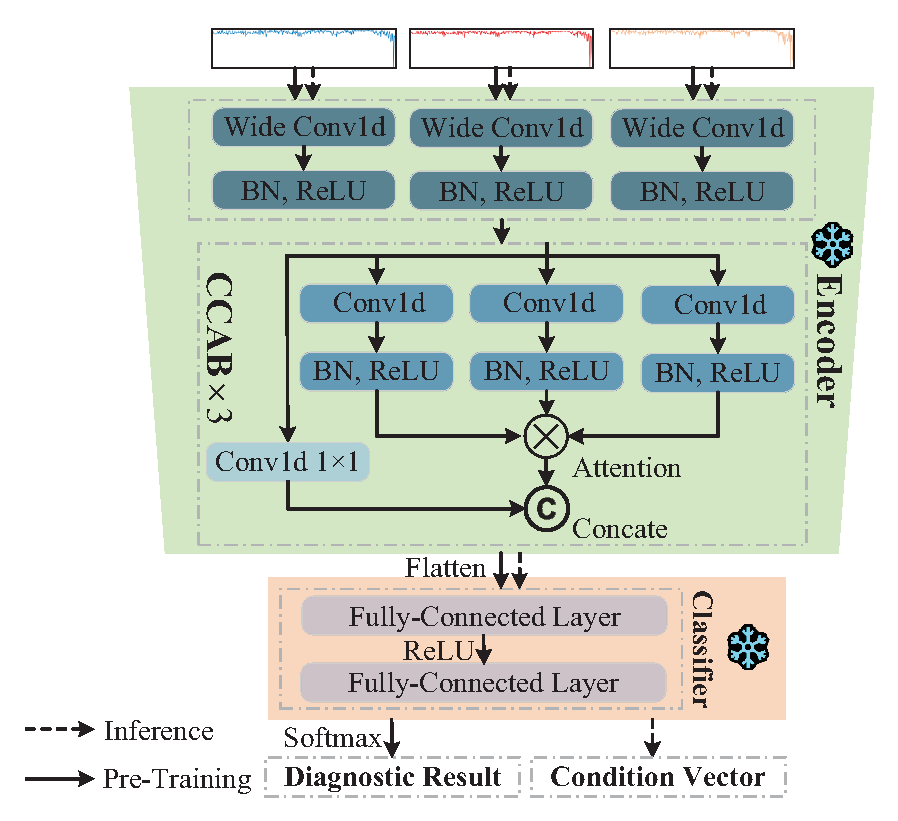
\includegraphics[width=\textwidth]{Img/DA-TMLLM_figures/trans/ControlNet.eps}
    \bicaption{DA-TMLLM~架构图}{Diagram of DA-TMLLM framework}
    \label{fig:controlnet}
\end{figure}

\begin{figure}[!htbp]
    \centering
    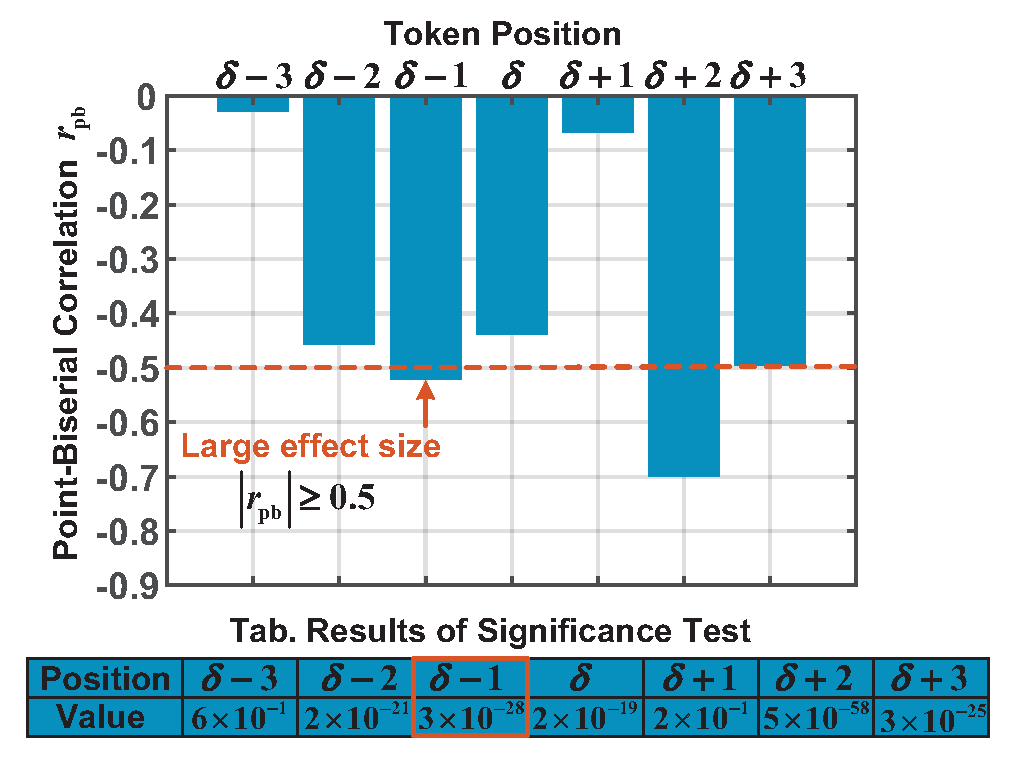
\includegraphics[width=\textwidth]{Img/DA-TMLLM_figures/trans/correlation.eps}
    \bicaption{DA-TMLLM~架构图}{Diagram of DA-TMLLM framework}
    \label{fig:correlation}
\end{figure}

\begin{figure}[!htbp]
    \centering
    
\includegraphics[width=\textwidth]{Img/DA-TMLLM_figures/trans/whole_strategy.eps}
    \bicaption{DA-TMLLM~架构图}{Diagram of DA-TMLLM framework}
    \label{fig:strategy}
\end{figure}

\section{实验评估}

\subsection{实验设置}

Peng等\cite{Peng_Liu_Du_Gao_Wang_2025}

\subsection{性能对比试验}

\begin{figure}[!htbp]
    \centering
    \begin{subfigure}[b]{0.35\textwidth}
      
\includegraphics[width=\textwidth]{oaspl_a}
      \caption{}
      \label{fig:oaspl_a}
    \end{subfigure}%
    ~%add desired spacing
    \begin{subfigure}[b]{0.35\textwidth}
      
\includegraphics[width=\textwidth]{oaspl_b}
      \caption{}
      \label{fig:oaspl_b}
    \end{subfigure}
    \begin{subfigure}[b]{0.35\textwidth}
      
\includegraphics[width=\textwidth]{oaspl_c}
      \caption{}
      \label{fig:oaspl_c}
    \end{subfigure}%
    ~%add desired spacing
    \begin{subfigure}[b]{0.35\textwidth}
      
\includegraphics[width=\textwidth]{oaspl_d}
      \caption{}
      \label{fig:oaspl_d}
    \end{subfigure}
    \bicaption{总声压级。(a) 这是子图说明信息，(b) 这是子图说明信息，(c) 这是子图说明信息，(d) 这是子图说明信息。}{OASPL.(a) This is the explanation of subfig, (b) This is the explanation of subfig, (c) This is the explanation of subfig, (d) This is the explanation of subfig.}
    \label{fig:oaspl}
\end{figure}

\subsection{消融实验}

\subsection{超参数敏感性分析}

\begin{figure}[!htbp]
    \centering
    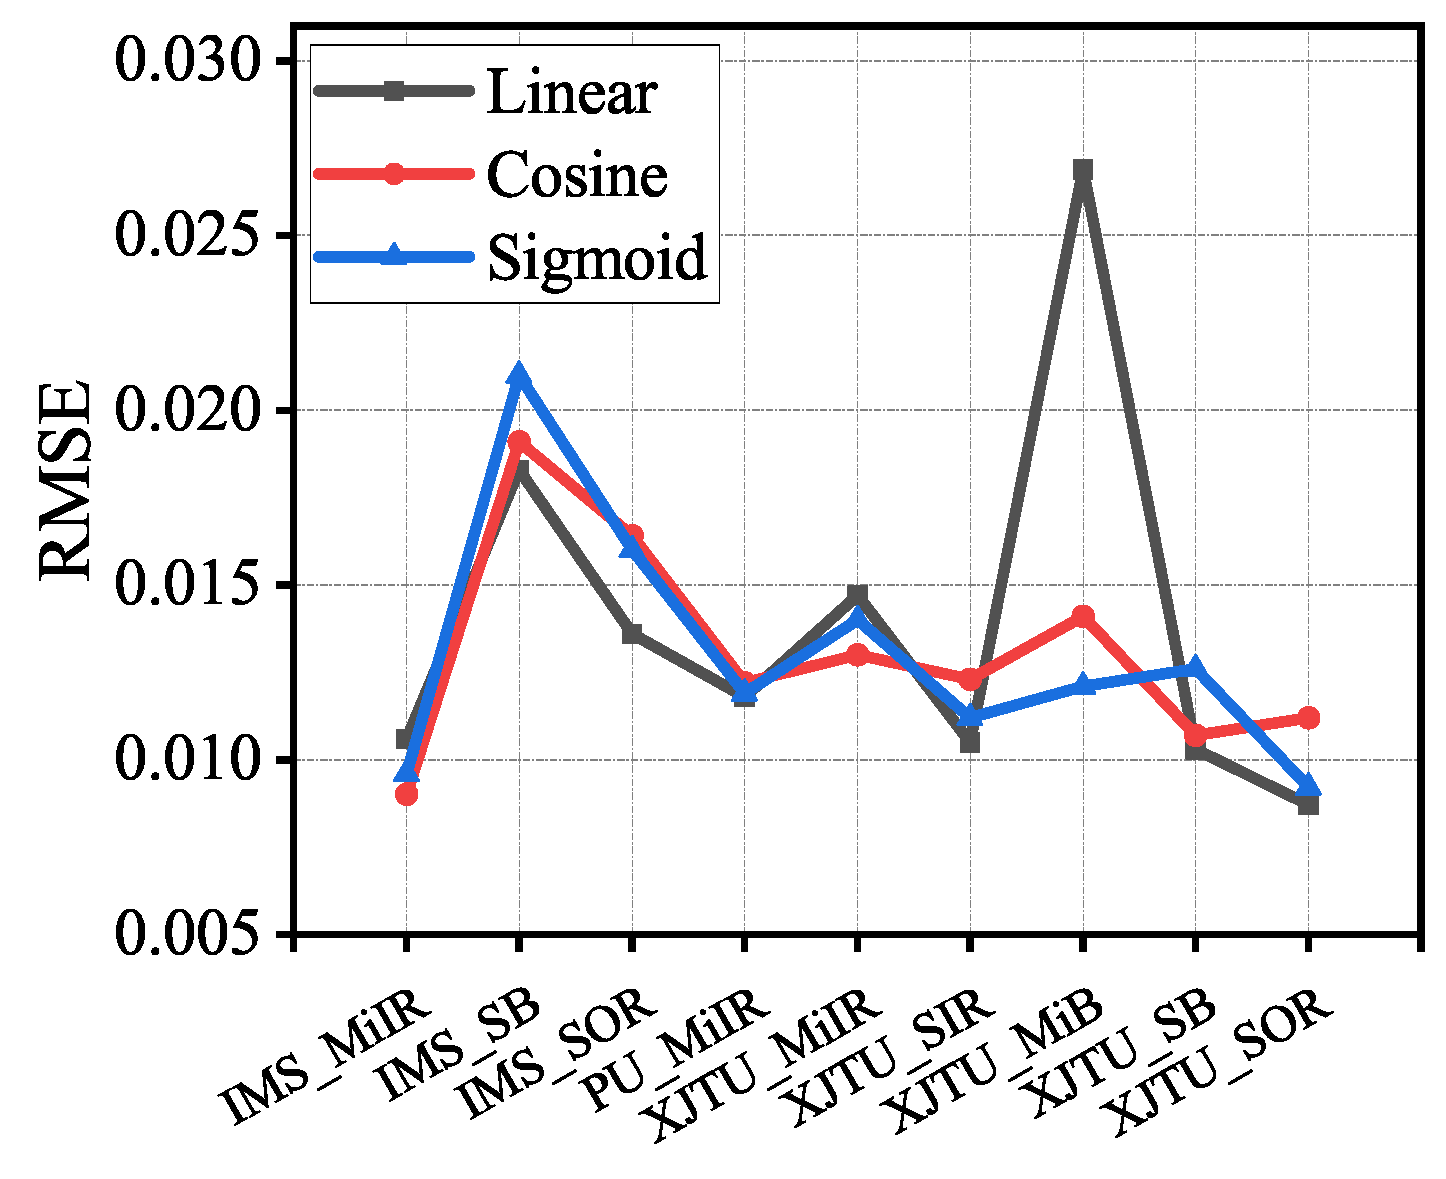
\includegraphics[width=\textwidth]{Img/DA-TMLLM_figures/trans/sa1.eps}
    \bicaption{DA-TMLLM~架构图}{Diagram of DA-TMLLM framework}
    \label{fig:sensitivity_sa1}
\end{figure}

\begin{figure}[!htbp]
    \centering
    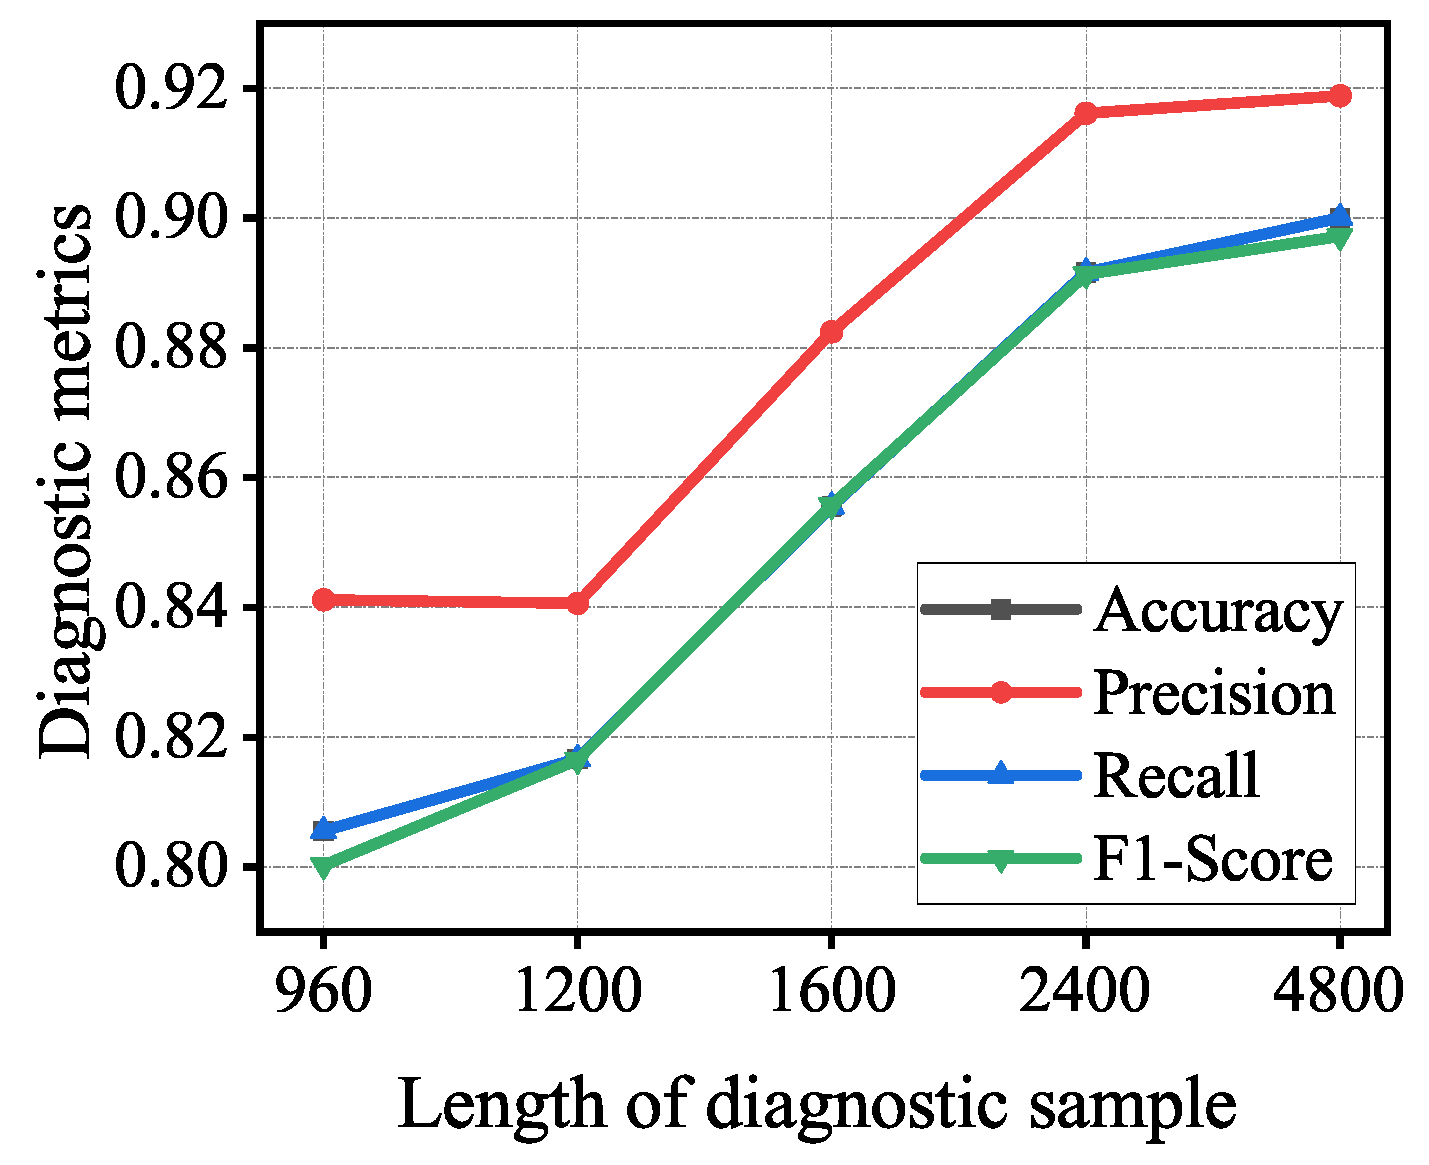
\includegraphics[width=\textwidth]{Img/DA-TMLLM_figures/trans/sa2.eps}
    \bicaption{DA-TMLLM~架构图}{Diagram of DA-TMLLM framework}
    \label{fig:sensitivity_sa2}
\end{figure}

\begin{figure}[!htbp]
    \centering
    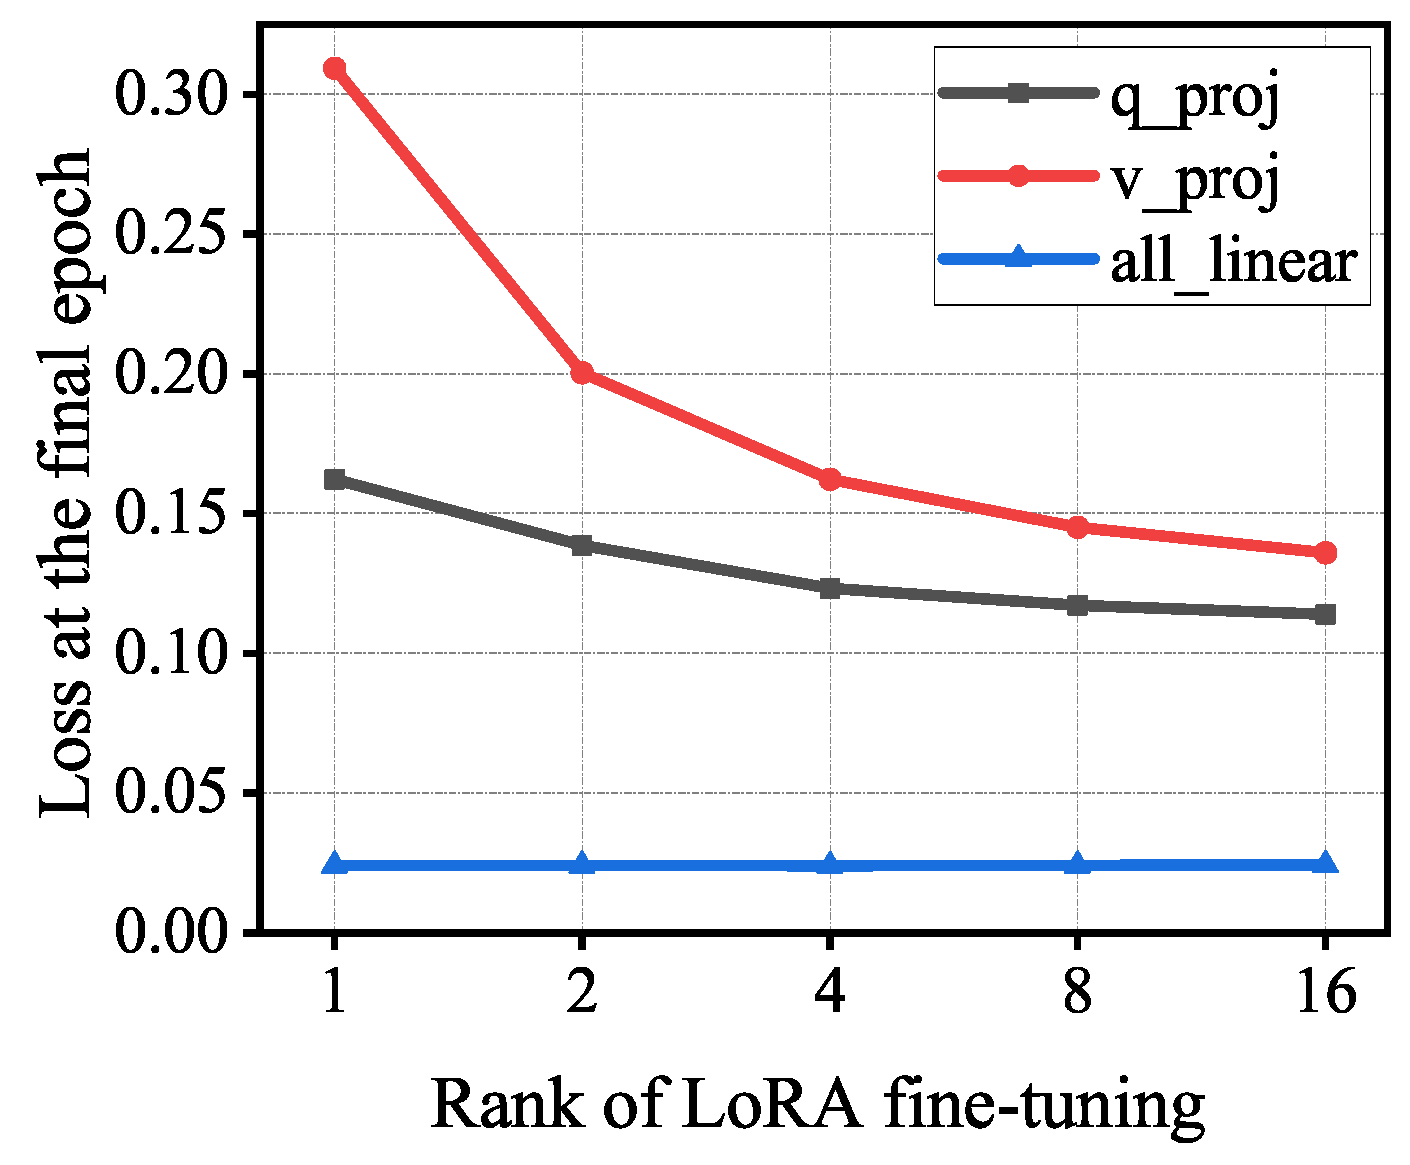
\includegraphics[width=\textwidth]{Img/DA-TMLLM_figures/trans/sa3.eps}
    \bicaption{DA-TMLLM~架构图}{Diagram of DA-TMLLM framework}
    \label{fig:sensitivity_sa3}
\end{figure}

\begin{figure}[!htbp]
    \centering
    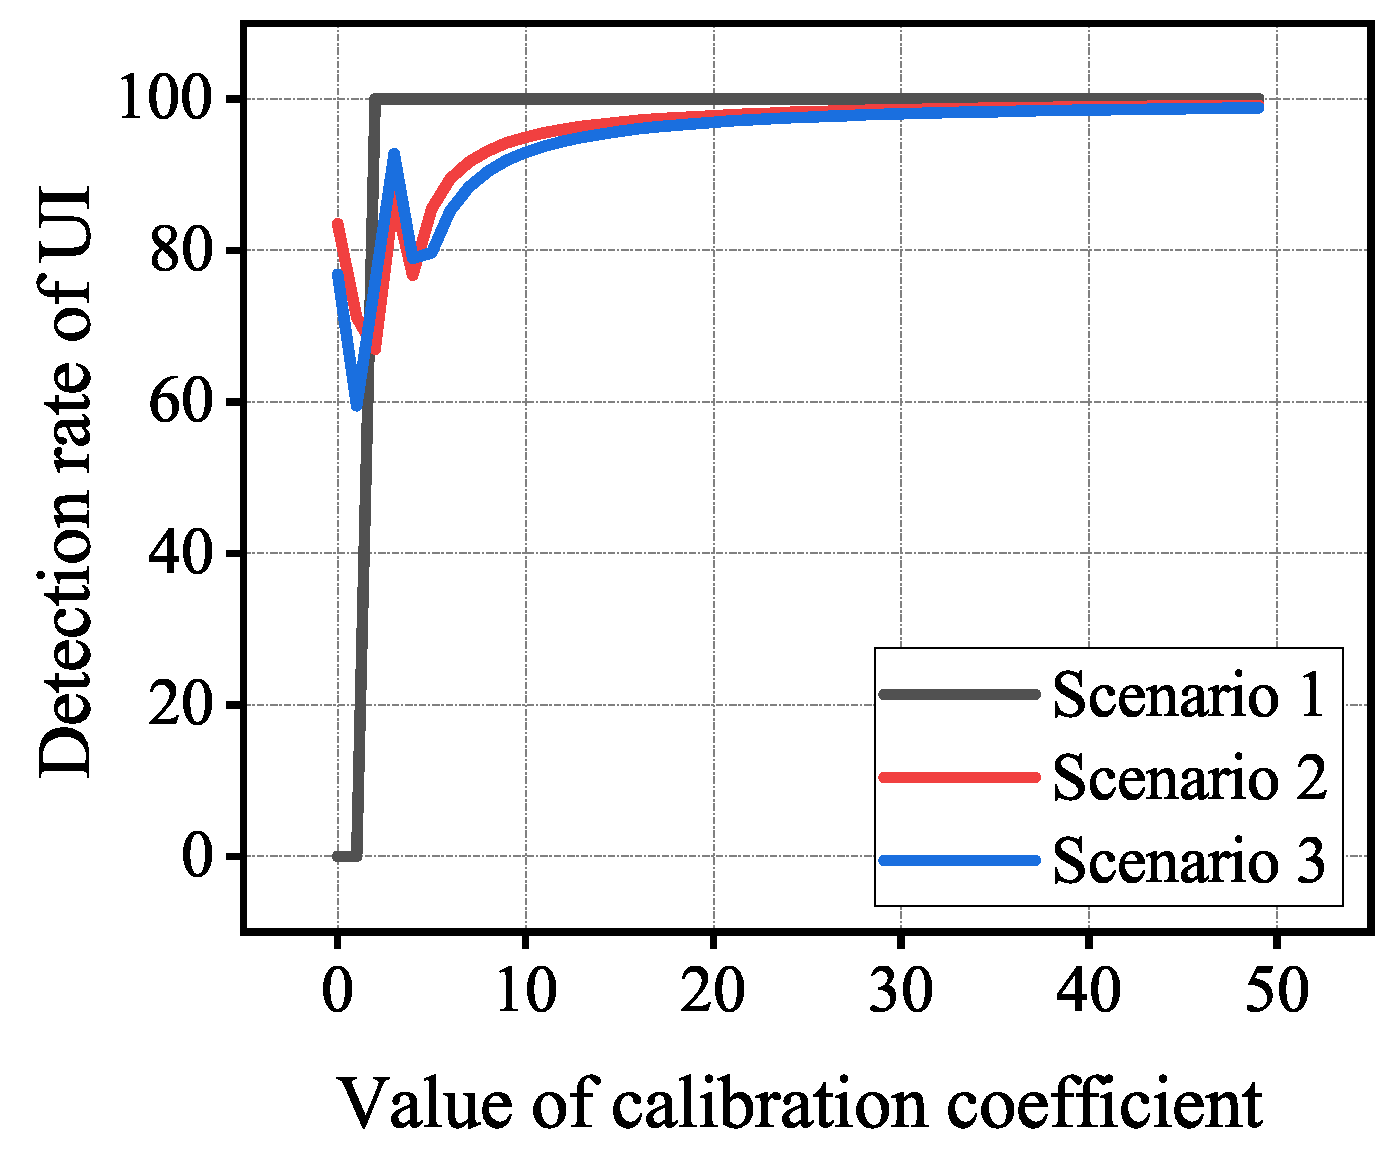
\includegraphics[width=\textwidth]{Img/DA-TMLLM_figures/trans/sa4.eps}
    \bicaption{DA-TMLLM~架构图}{Diagram of DA-TMLLM framework}
    \label{fig:sensitivity_sa4}
\end{figure}

\section{本章小结}